\documentclass[aspectratio=169,10pt]{beamer}
\usetheme{Madrid}
\usecolortheme{default}
\setbeamertemplate{navigation symbols}{}
\setbeamertemplate{footline}[frame number]

\usepackage{amsmath,amssymb}
\usepackage{graphicx}
\usepackage{booktabs}
\usepackage{listings}
\usepackage{xcolor}

\graphicspath{{./}}   % all images are in the same doc/ directory

\lstset{
  basicstyle=\ttfamily\tiny,
  keywordstyle=\color{blue},
  commentstyle=\color{gray},
  breaklines=true,
  frame=single,
  backgroundcolor=\color{gray!8},
}

\title{1D Helmholtz EM Solver}
\subtitle{Design, Validation, and Applications}
\author{Zhiping Li \and Xuyang Xu\\[4pt]
  \small\texttt{zl8336@princeton.edu}}
\institute{APC 523 Final Project}
\date{}

% ─────────────────────────────────────────────
\begin{document}

\begin{frame}
  \titlepage
\end{frame}

% ── Slide 1: Problem overview ─────────────────
\begin{frame}{Problem Overview}
  \textbf{Goal:} solve 1D Helmholtz equation for monochromatic EM scattering at a
  dielectric transition layer.

  \vspace{4pt}
  \begin{columns}[T]
    \column{0.48\textwidth}
      \textbf{Domain}\\[2pt]
      \begin{tabular}{lll}
        \toprule
        Zone & Range & Medium \\
        \midrule
        Region 1    & $z \le z_1$ & uniform $\varepsilon_1$ \\
        Transition  & $z_1 \le z \le z_2$ & $\varepsilon_r(z)$ \\
        Region 2    & $z \ge z_2$ & uniform $\varepsilon_2$ \\
        \bottomrule
      \end{tabular}

      \vspace{6pt}
      \textbf{Sign convention:} $e^{-j\omega t}$; right-going $\propto e^{-jk_z z}$\\
      $k_x = k_0\sqrt{\varepsilon_1}\sin\theta$ (conserved)

    \column{0.48\textwidth}
      \textbf{TE (S):}
      \[
        \frac{d^2 E_y}{dz^2} + \bigl[k_0^2\varepsilon_r(z) - k_x^2\bigr]E_y = 0
      \]

      \textbf{TM (P):}
      \[
        \frac{d^2 H_y}{dz^2}
        - \frac{1}{\varepsilon_r}\frac{d\varepsilon_r}{dz}\frac{dH_y}{dz}
        + \bigl[k_0^2\varepsilon_r(z) - k_x^2\bigr]H_y = 0
      \]
  \end{columns}
\end{frame}

% ── Slide 2: Numerical methods ────────────────
\begin{frame}{Two Independent Numerical Methods}
  \begin{columns}[T]
    \column{0.52\textwidth}
      \begin{tabular}{lll}
        \toprule
        Method & Back-end & Order \\
        \midrule
        ODE shooting & diffrax / JAX GPU & 5th (Dopri5) \\
        FEM (P1/P2)  & JAX dense solver  & 2nd / 4th \\
        \bottomrule
      \end{tabular}

      \vspace{6pt}
      \textbf{ODE solvers available:}
      \begin{tabular}{lll}
        \toprule
        Solver & Family & Order \\
        \midrule
        \texttt{Heun}              & Explicit RK       & 2 \\
        \texttt{Tsit5}             & Explicit RK (FSAL)& 5 \\
        \texttt{Dopri5}            & Explicit RK (FSAL)& 5 \\
        \texttt{KenCarp4}          & IMEX ARK          & 4 \\
        \texttt{SemiImplicitEuler} & Symplectic        & 1 \\
        \bottomrule
      \end{tabular}

    \column{0.45\textwidth}
      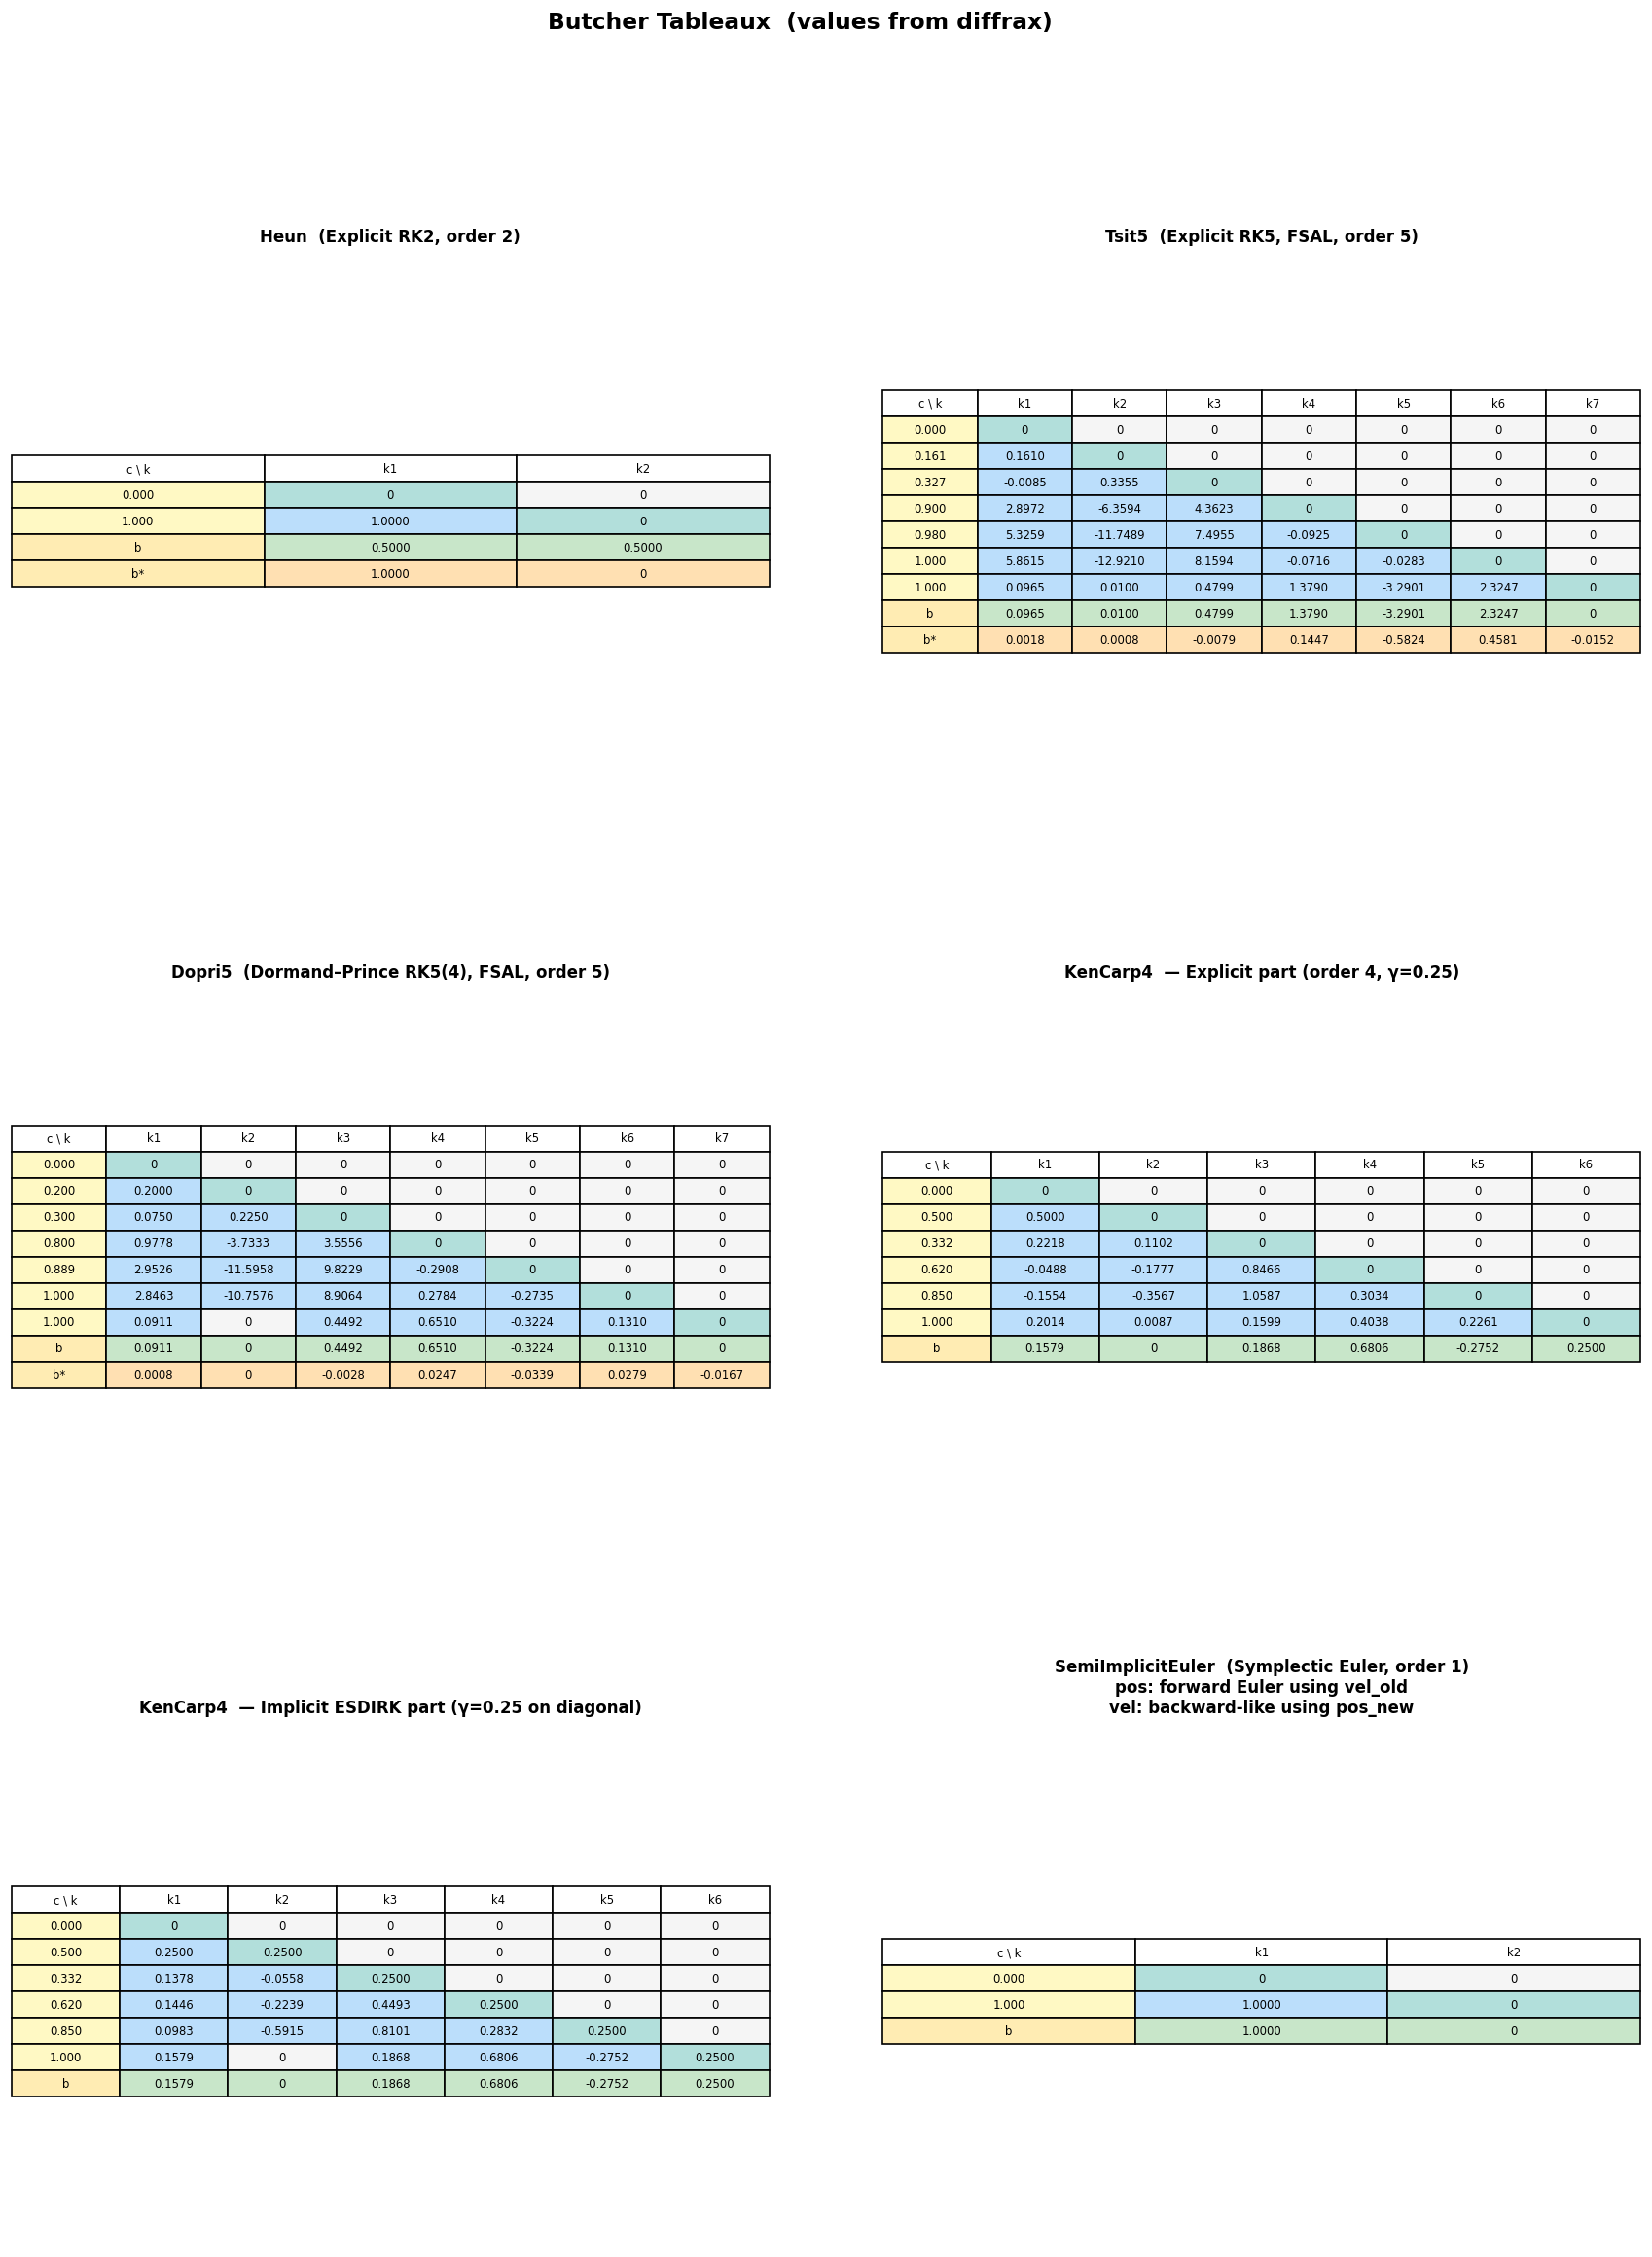
\includegraphics[width=\linewidth]{butcher_tableaux.png}
      \vspace{2pt}
      {\footnotesize Butcher tableaux for explicit RK solvers.}
  \end{columns}

  \vspace{4pt}
  \textbf{Default resolution:}
  ODE $= 50\times\max\sqrt{|\varepsilon_r|}$ cells/$\lambda_0$;
  FEM $= 100\times\max\sqrt{|\varepsilon_r|}$;
  exterior $=$ res\_trans$/2$.
\end{frame}

% ── Slide 3: Basic usage ──────────────────────
\begin{frame}[fragile]{Basic Usage}
\begin{lstlisting}[language=Python]
from main import HelmholtzSolver1D
import numpy as np

def eps_tanh(z, eps1=1.0, eps2=4.0, zc=0.0, delta=0.33):
    return (eps1+eps2)/2 + (eps2-eps1)/2 * np.tanh((z-zc)/delta)

solver = HelmholtzSolver1D(eps_tanh, z1=-1.0, z2=+1.0,
                           theta_deg=45.0, pol='S', lambda0=1.0)
result_ode = solver.solve_ode()
result_fem = solver.solve_fem(res_trans=200, res_ext=100, order=2)
solver.energy_check(result_ode['r'], result_ode['t'])   # R+T should be ~1
solver.plot_field(result_ode)
\end{lstlisting}

  \begin{columns}[T]
    \column{0.48\textwidth}
      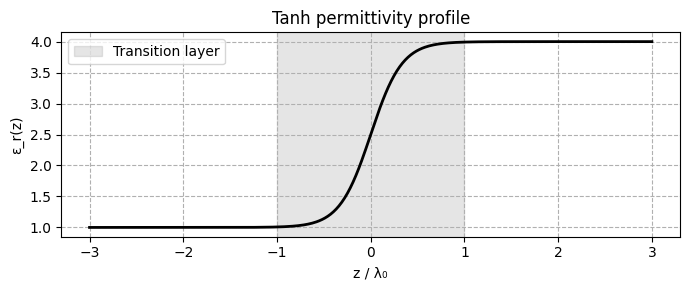
\includegraphics[width=\linewidth]{Tanh_permittivity_profile.png}
      \centering{\footnotesize Tanh $\varepsilon_r(z)$, $\varepsilon_1{=}1$, $\varepsilon_2{=}4$}
    \column{0.48\textwidth}
      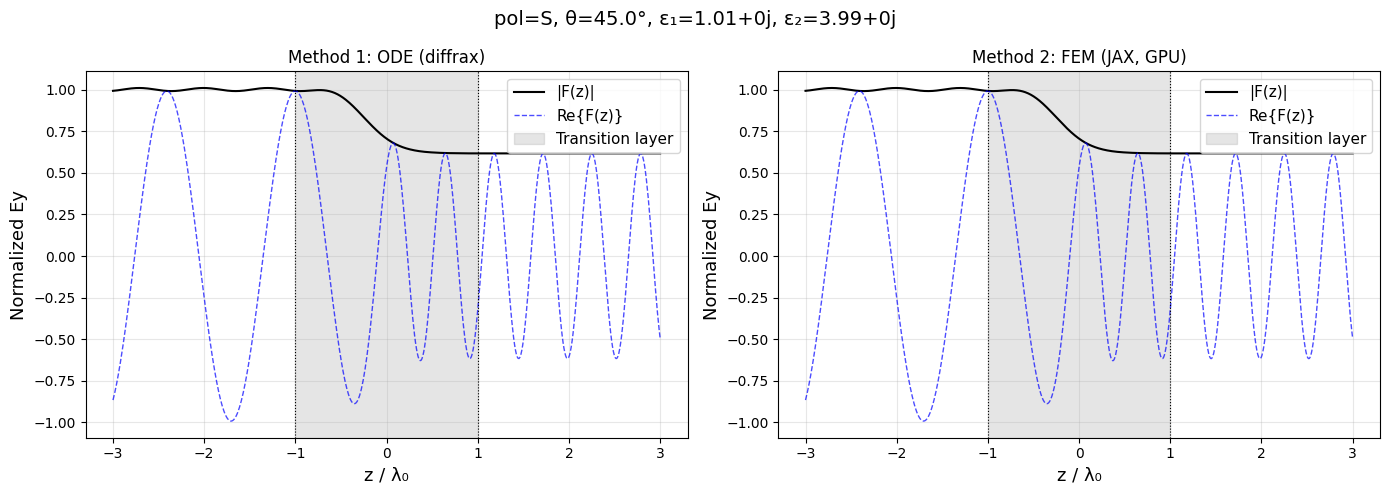
\includegraphics[width=\linewidth]{Tanh_Field.png}
      \centering{\footnotesize Field profile, $\theta{=}45°$, TE}
  \end{columns}
\end{frame}

% ── Slide 4: Airy setup ───────────────────────
\begin{frame}{Correctness: Airy Analytical Benchmark}
  \textbf{V-shaped profile} (piecewise-linear):
  \[
    \varepsilon_r(z) = \varepsilon_0 + (1-\varepsilon_0)\,|z/\delta|,\quad
    |z|\le\delta;\qquad \varepsilon_r=1,\quad |z|>\delta
  \]
  TE equation $\to$ Airy equation $\Rightarrow$ exact closed-form solution in
  $\mathrm{Ai}(\xi)$, $\mathrm{Bi}(\xi)$.

  \vspace{4pt}
  Two test cases ($\delta = 2\lambda_0$):
  \begin{itemize}
    \item $\varepsilon_0 = 5$: dielectric, no turning points
    \item $\varepsilon_0 = -3$: metallic core, turning points at $|z|=3\delta/4$
  \end{itemize}

  \begin{center}
    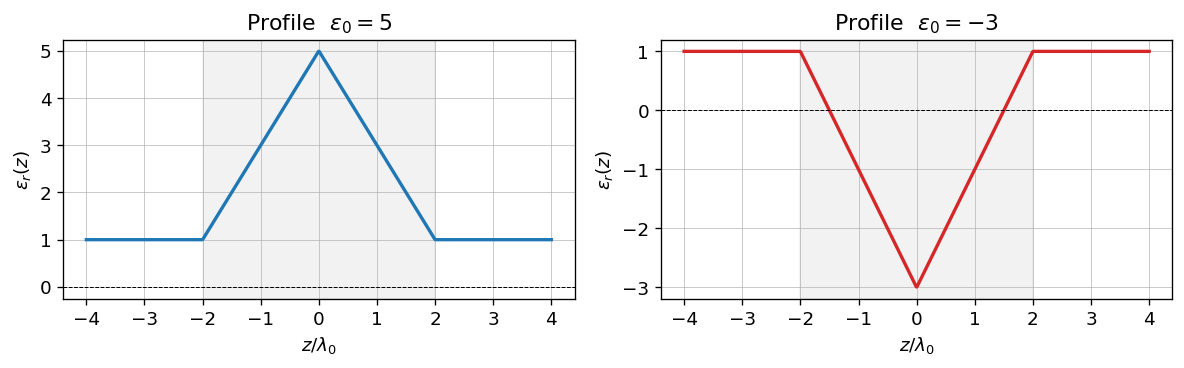
\includegraphics[width=0.7\linewidth]{profile.png}\\
    {\footnotesize V-shaped $\varepsilon_r(z)$ profiles for both test cases.}
  \end{center}
\end{frame}

% ── Slide 5: Convergence results ─────────────
\begin{frame}{Correctness: Convergence Results ($\theta=45°$, TE)}
  \begin{columns}[T]
    \column{0.48\textwidth}
      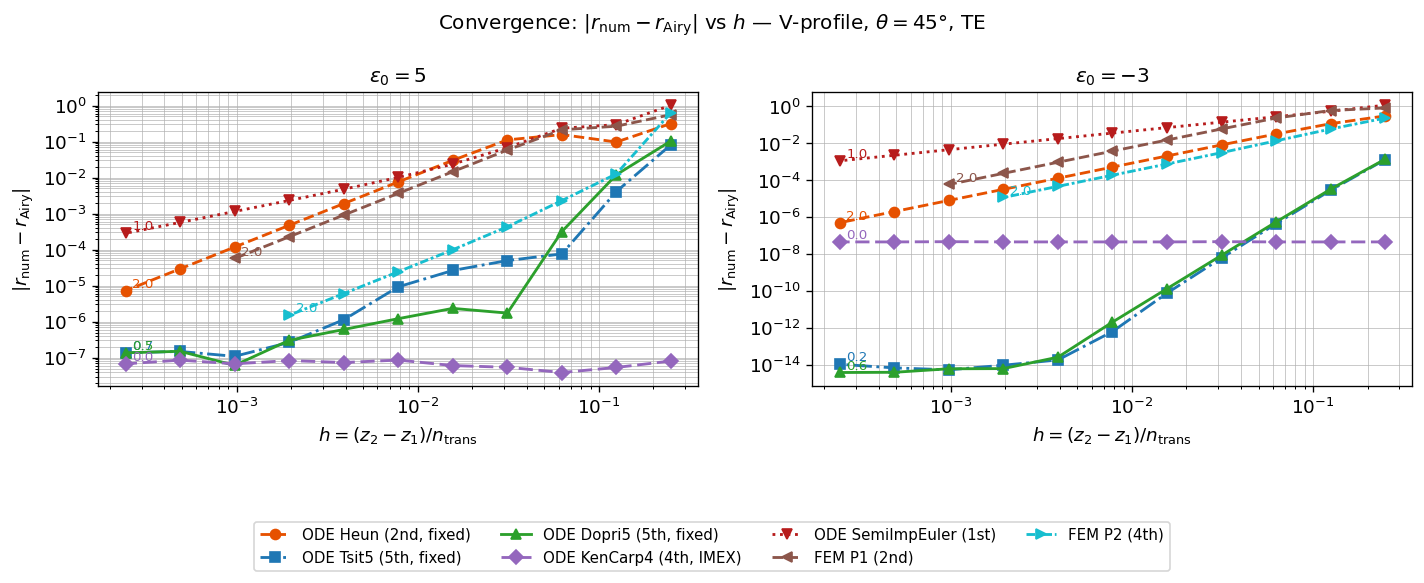
\includegraphics[width=\linewidth]{conv_r_error.png}\\
      {\footnotesize $|r_\text{num}-r_\text{Airy}|$ vs step size $h$.}
    \column{0.48\textwidth}
      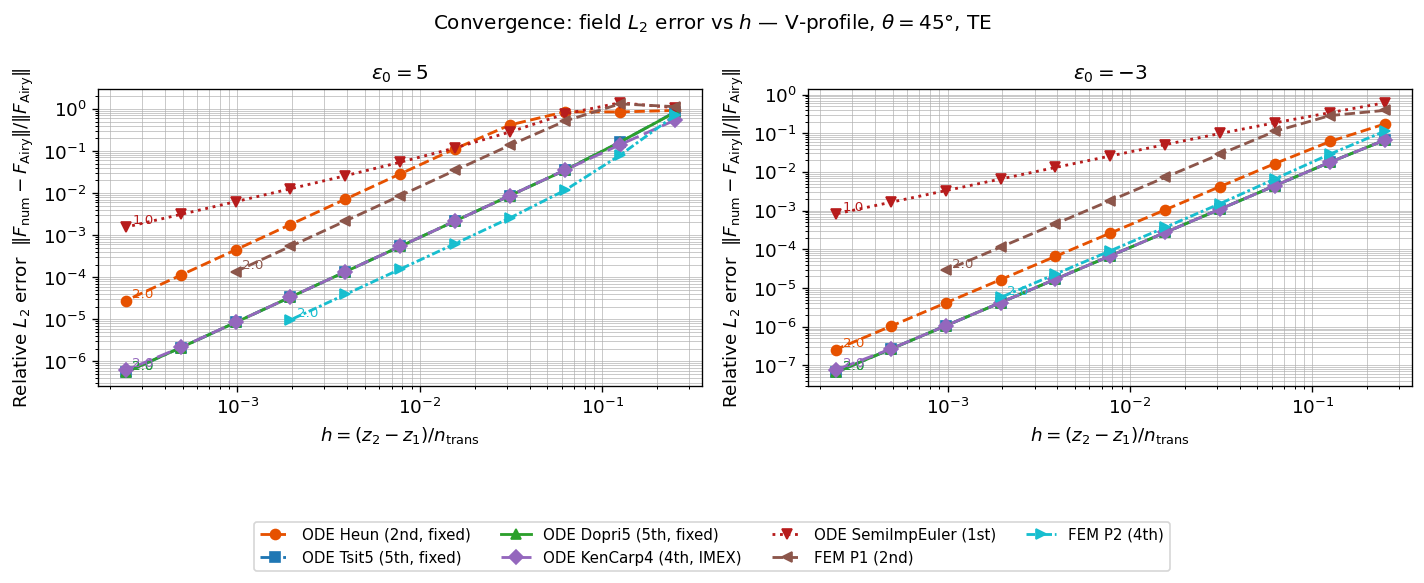
\includegraphics[width=\linewidth]{conv_l2_error.png}\\
      {\footnotesize Field $L_2$ error vs $h$.}
  \end{columns}

  \vspace{4pt}
  \begin{itemize}\small
    \item \textbf{$r$ error:} SemiImplEuler slope~1; Heun/FEM~P1/P2 slope~2;
          Dopri5/Tsit5 slope~4 then flattens; KenCarp4 flat (IMEX splitting error).
    \item \textbf{$L_2$ error:} all methods except SemiImplEuler converge at slope~2
          (limited by 2nd-order quadrature of the norm).
    \item \textbf{Absolute accuracy:} FEM~P2 is $\sim10^2\times$ more accurate than P1
          at the same $h$; ODE methods match FEM~P2 at far coarser resolution.
          FEM~P2 at fine mesh demands tens of GB --- ODE is preferred for high accuracy.
    \item At default ODE resolution ($50\sqrt{5}\approx112$ cells/$\lambda_0$):
          $|r_\text{num}-r_\text{Airy}| < 10^{-5}$.
  \end{itemize}
\end{frame}

% ── Slide 6: Stability ────────────────────────
\begin{frame}{Stability Near a Dielectric Zero-Crossing}
  \textbf{Setup:} $\varepsilon_0=-3$, $\delta=2\lambda_0$, $\theta=45°$,
  resolution swept 4–512 cells/$\lambda_0$.\\[4pt]
  \textbf{TE:} classical turning point ($R=1$ exactly from Airy).\\
  \textbf{TM:} $(1/\varepsilon_r)(d\varepsilon_r/dz)$ diverges at $\varepsilon_r=0$
  $\Rightarrow$ regularise $\varepsilon_r \to \varepsilon_r+j\eta$, $\eta=10^{-4}$.

  \begin{center}
    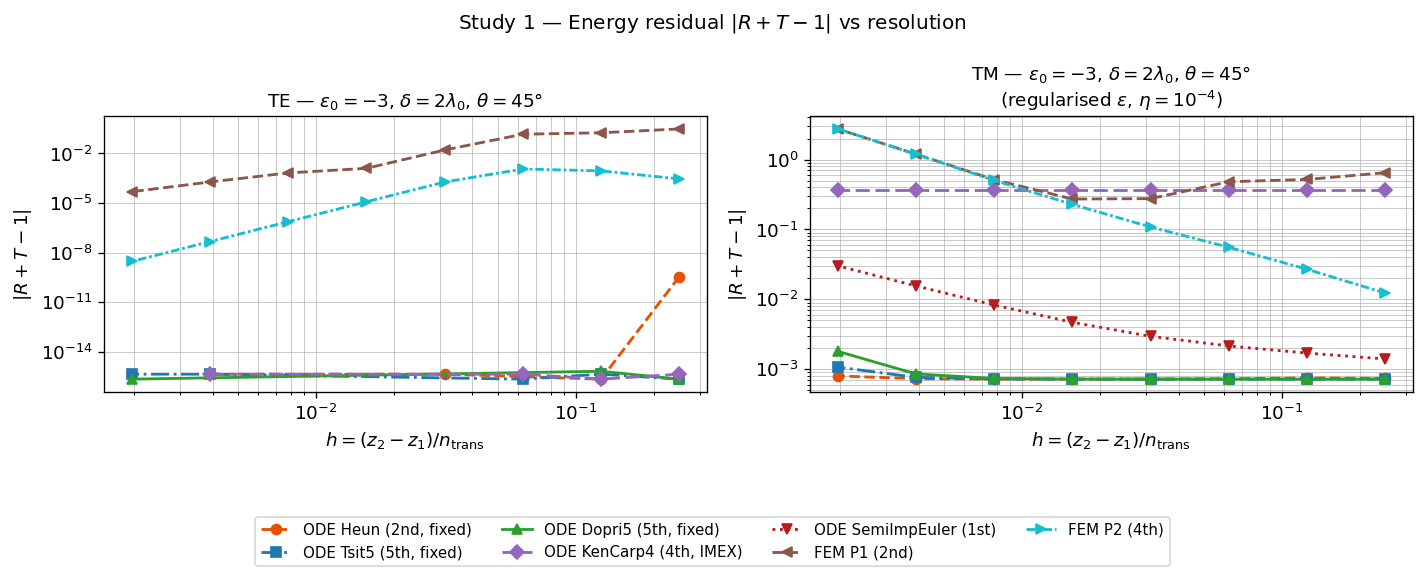
\includegraphics[width=0.55\linewidth]{stab1_energy.png}\\
    {\footnotesize Energy residual $|R+T-1|$ vs resolution.
      Left: TE.  Right: TM with $j\eta$ regularisation.}
  \end{center}

  \begin{itemize}\footnotesize
    \item \textbf{TE:} all methods reach floating-point energy conservation;
          ODE $|R+T-1|\lesssim10^{-14}$; FEM improves with $h$, P2 $>$ P1.
    \item \textbf{TM:} fixed-step ODE stalls at $\sim10^{-3}$; KenCarp4 flat at $\sim0.5$.
    \item All TM methods \emph{worsen} at finer $h$; FEM~P2 gives $|R+T-1|>1$
          for $h<10^{-2}\lambda_0$ --- $j\eta$ regularisation insufficient;
          reformulation ($u=H_y/\varepsilon_r$) needed.
  \end{itemize}
\end{frame}

% ── Slide 7: GPU efficiency ───────────────────
\begin{frame}{Efficiency: GPU-Parallel Parameter Sweeps}
  Built on \textbf{JAX} (64-bit complex); GPU via \texttt{jax\_platform\_name='gpu'}.\\
  \texttt{sweep\_ode}/\texttt{sweep\_fem}: vectorise over $\theta$ array with
  \texttt{jax.vmap} $\Rightarrow$ single GPU kernel. \textbf{10--50$\times$ speedup}
  vs Python loop.

  \vspace{4pt}
  \textbf{Example:} $R(\theta)$ for tanh transition
  $\varepsilon_r(z)=\frac{\varepsilon_1+\varepsilon_2}{2}+\frac{\varepsilon_2-\varepsilon_1}{2}
  \tanh(z/\delta)$, $\varepsilon_1{=}1$, $\varepsilon_2{=}4$,
  $\delta$ swept over 8 values $0.01\lambda_0$–$2\lambda_0$.

  \begin{center}
    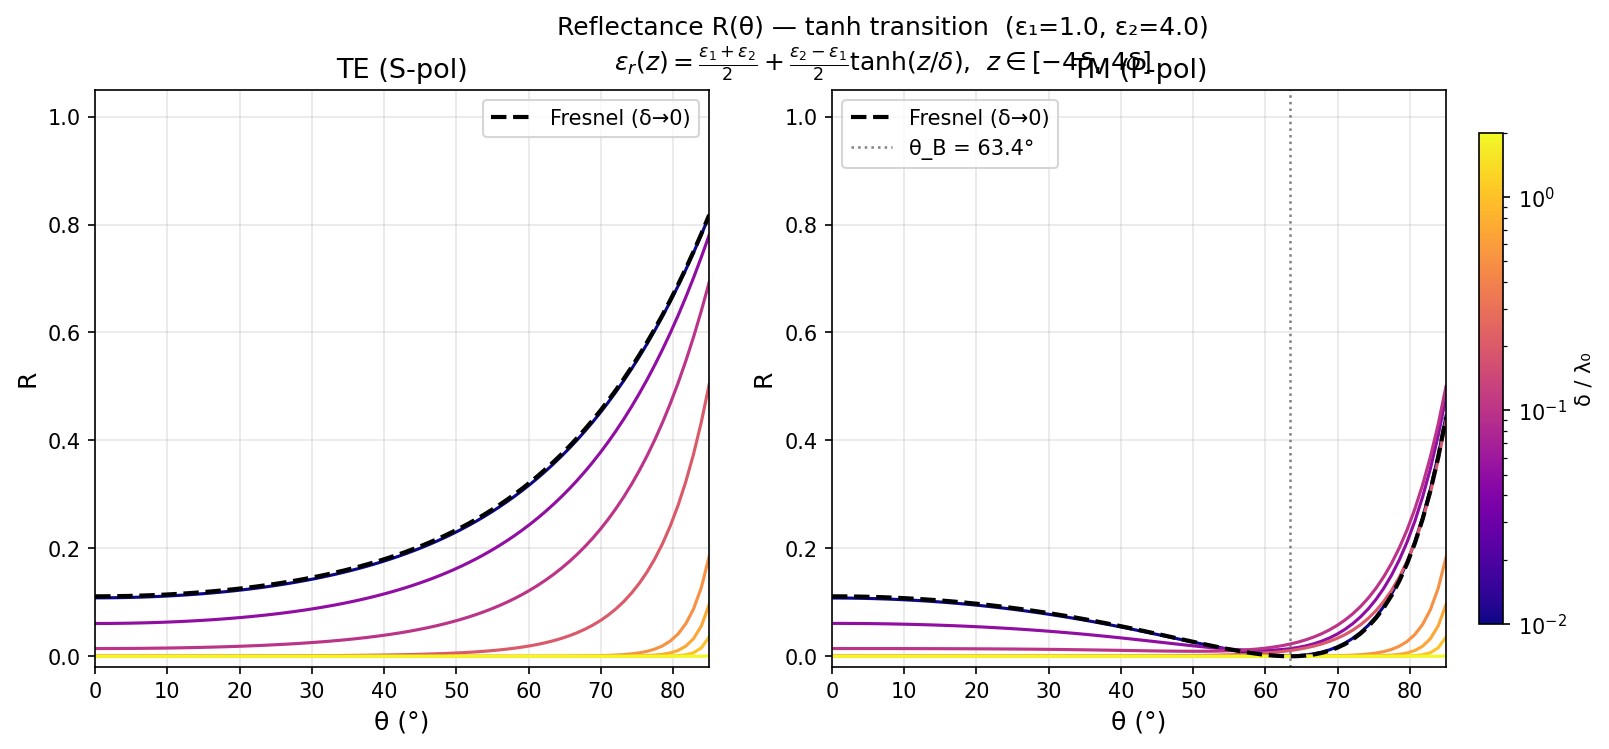
\includegraphics[width=0.55\linewidth]{gradient_R_vs_theta.png}\\
    {\footnotesize Reflectance $R(\theta)$ for TE (left) and TM (right), coloured by $\delta$.
    Black dashed: sharp-interface Fresnel limit.}
  \end{center}

  \begin{itemize}\small
    \item TE: reflectance suppressed monotonically as $\delta$ increases.
    \item TM: Brewster angle $\theta_B\approx63.4°$ ($\varepsilon_2/\varepsilon_1=4$)
          preserved for all $\delta$.
    \item Both polarisations recover the Fresnel limit as $\delta\to0$
          --- independent cross-check that TE and TM are both correctly implemented.
  \end{itemize}
\end{frame}

% ── Slide 8: Plasma application ───────────────
\begin{frame}{Application: Plasma Density Diagnostics}
  \begin{columns}[T]
    \column{0.48\textwidth}
      \textbf{Profile} (linear ramp into plasma):
      \[
        \varepsilon_r(z)=\begin{cases}1 & z<-\delta\\-z/\delta & |z|\le\delta\\-1&z>\delta\end{cases}
      \]
      $\varepsilon_r$ crosses zero at $z=0$.  Because $\varepsilon_2<0$, $|r|^2=1$ and
      \textbf{phase} $\angle r$ carries all information about the density gradient $\delta$.

      \vspace{4pt}
      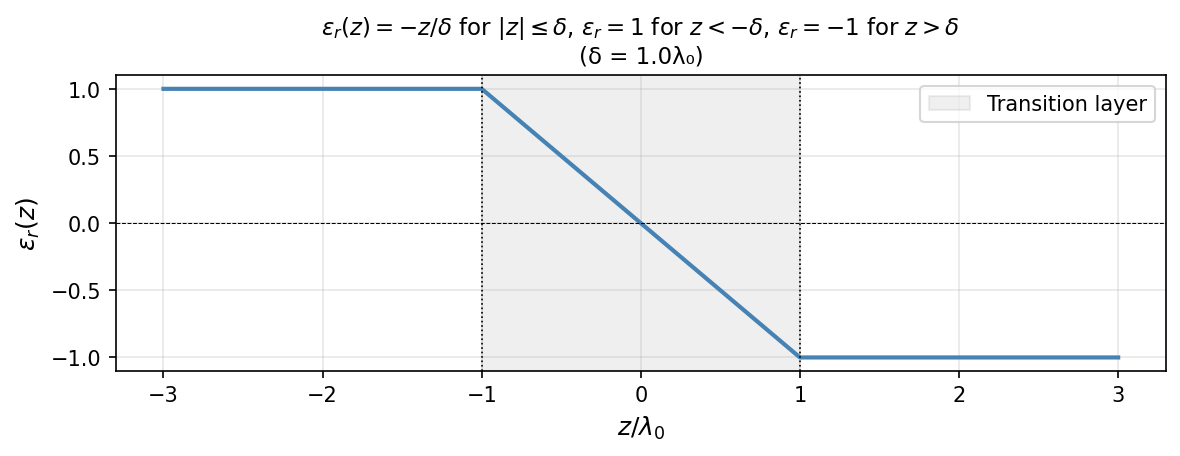
\includegraphics[width=\linewidth]{plasma_eps_profile.png}\\
      {\footnotesize $\varepsilon_r(z)$ for $\delta=\lambda_0$.}

    \column{0.48\textwidth}
      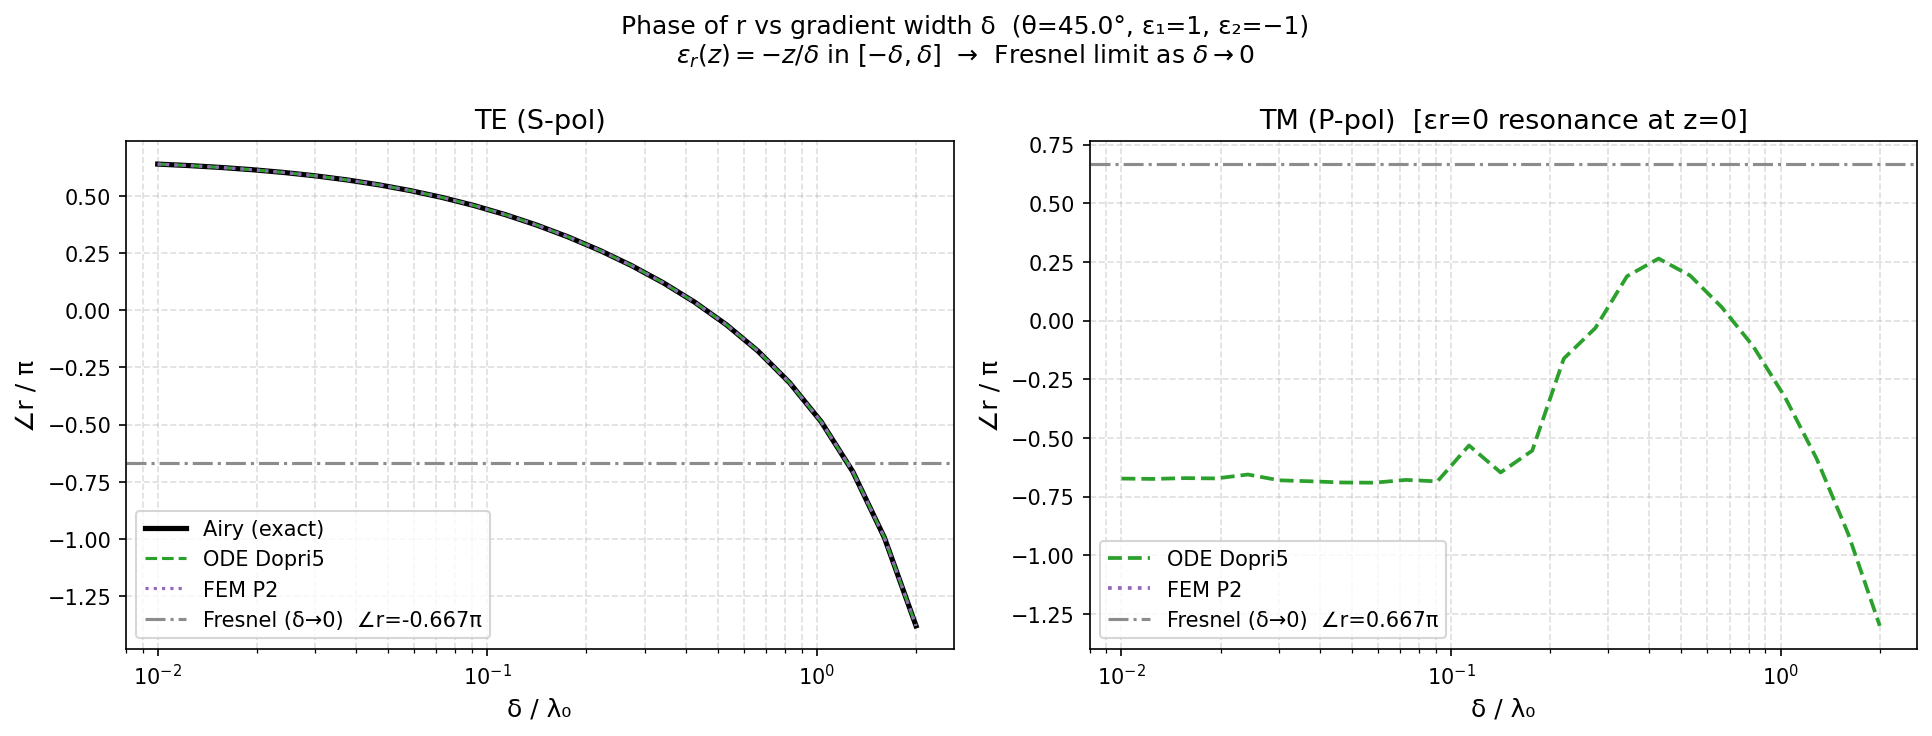
\includegraphics[width=\linewidth]{plasma_phase_vs_delta.png}\\
      {\footnotesize $\angle r$ vs $\delta$, $\theta=45°$.}

      \vspace{4pt}
      \begin{itemize}\small
        \item ODE (TE) agrees with Airy across full $\delta$ range.
        \item FEM result not yet correct for this profile (open issue).
        \item \textbf{Prospect:} infer $\delta$ from measured $\angle r$:
          $\delta_\text{infer}=\arg\min_\delta|\angle r_\text{meas}-\angle r_\text{ODE}|^2$\\
          applicable to laser--plasma surface diagnostics.
      \end{itemize}
  \end{columns}
\end{frame}

% ── Slide 9: Bugs & fixes ─────────────────────
\begin{frame}{Known Bugs and Fixes}
  \textbf{Bug 1: Exponential growth for evanescent transmitted wave ($\varepsilon_2<0$)}

  \begin{columns}[T]
    \column{0.55\textwidth}
      \textit{Root cause:} branch cut $\mathrm{Im}(k_z)\ge0$ gives
      $k_{z2}=+j\alpha$ for plasma.  Na\"ive ansatz
      $F\propto e^{-jk_{z2}(z-z_2)}=e^{+\alpha(z-z_2)}\to\infty$.\\[4pt]
      \textit{Fix:} replace $k_{z2}\to\overline{k_{z2}}$ everywhere it appears as
      an outgoing BC (ODE IC, FEM Robin BC, field reconstruction, Airy BC).
      Backward-compatible: $k_{z2}\in\mathbb{R}$ for propagating waves.\\[4pt]
      \textit{Subtlety:} energy check $|r|^2=1$ does \emph{not} catch this bug ---
      only the field profile and $\angle r$ are corrupted.

    \column{0.42\textwidth}
      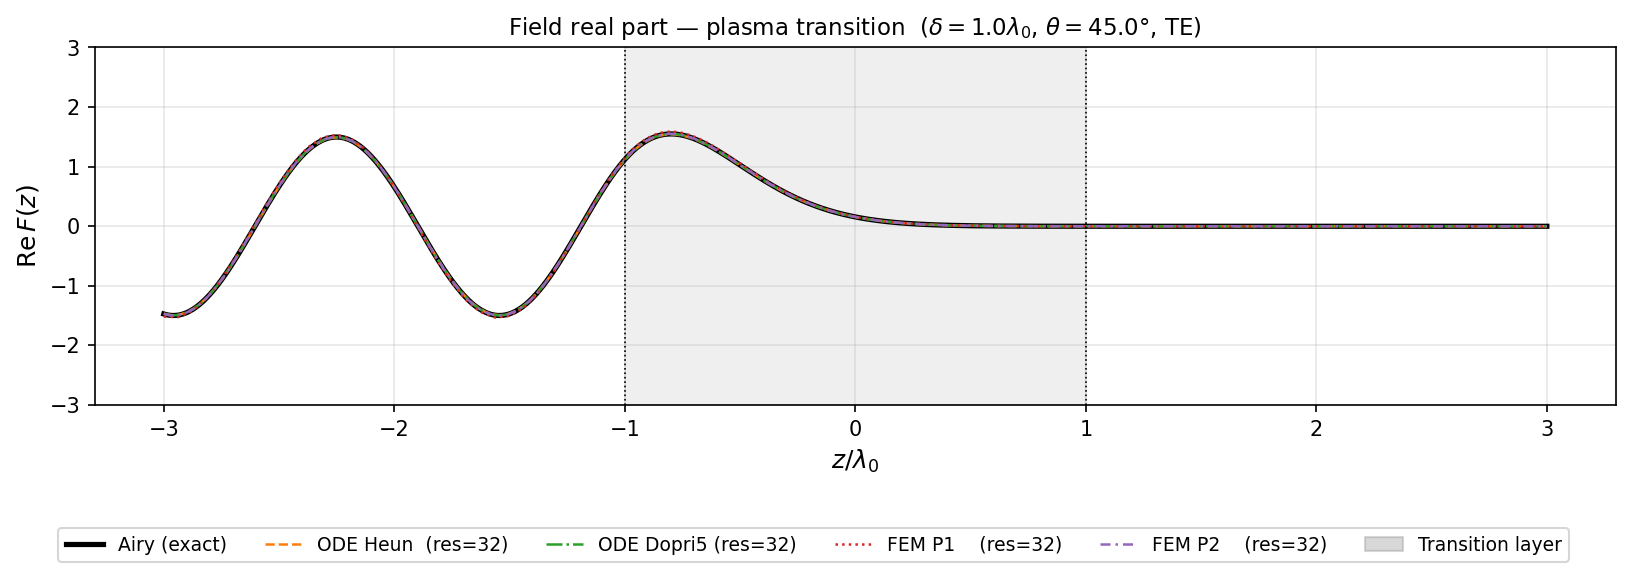
\includegraphics[width=\linewidth]{plasma_field_real.png}\\
      {\footnotesize $\mathrm{Re}\,F(z)$ after fix: field decays for $z>\delta$.}
  \end{columns}

  \vspace{8pt}
  \textbf{Bug 2: TM instability at $\varepsilon_r=0$}\\
  \textit{Root cause:} drift term $(1/\varepsilon_r)(d\varepsilon_r/dz)$ diverges.\\
  \textit{Fix:} $\varepsilon_r\to\varepsilon_r+j\eta$ ($\eta=10^{-4}$) shifts pole off real axis.
  Energy residual converges to floor $\propto\eta$; no blow-up.
\end{frame}

% ── Slide 10: Limitations & future work ───────
\begin{frame}{Current Limitations and Future Work}
  \textbf{Validation asymmetry}
  \begin{itemize}
    \item TE: fully characterised against Airy exact solution.
    \item TM: verified only by internal consistency (energy check, ODE--FEM agreement);
          no closed-form reference exists for general $\varepsilon_r(z)$.
  \end{itemize}

  \vspace{4pt}
  \textbf{Open questions for TM near $\varepsilon_r=0$}
  \begin{enumerate}\small
    \item Optimal $\eta$: trade-off between numerical stability and physical phase distortion.
    \item Reformulation $u=H_y/\varepsilon_r$ removes singularity analytically.
    \item Turning-point asymptotics for the irregular singular point.
  \end{enumerate}

  \vspace{4pt}
  \textbf{Planned extensions}\\[2pt]
  \begin{tabular}{lll}
    \toprule
    Feature & Status & Note \\
    \midrule
    Gradient-based inversion (autodiff) & Planned
      & FEM Jacobian via \texttt{jax.grad(jnp.linalg.solve)} \\
    TM analytical reference & In progress
      & Riemann--Green function \\
    FEM for plasma profile   & Open issue
      & $\varepsilon_r=0$ crossing destabilises assembly \\
    2D / anisotropic media   & Future
      & Coupled TE--TM \\
    \bottomrule
  \end{tabular}
\end{frame}

\end{document}
